\documentclass[tikz,border=2mm]{standalone}
\usetikzlibrary{shapes.geometric, arrows, positioning}
\begin{document}
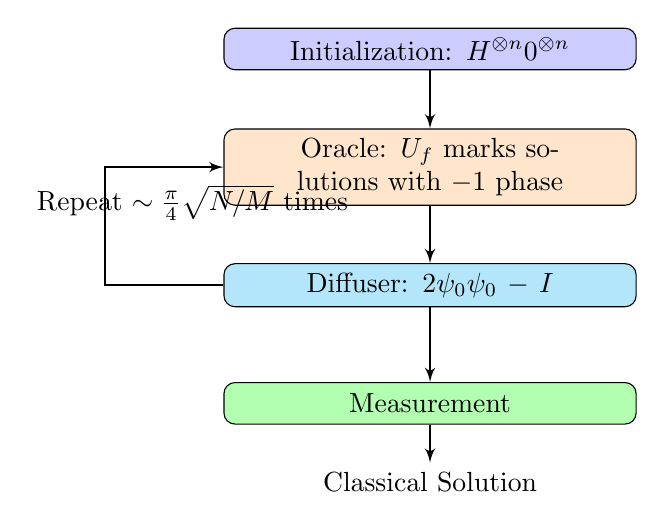
\begin{tikzpicture}[
    node distance=1.5cm,
    block/.style={rectangle, draw, fill=blue!20, text width=5cm, text centered, rounded corners, minimum height=1.5em},
    decision/.style={rectangle, draw, fill=orange!20, text width=5cm, text centered, rounded corners, minimum height=1.5em},
    line/.style={draw, -latex', thick}
]

\node [block] (init) {Initialization: $H^{\otimes n} \ket{0}^{\otimes n}$};
\node [decision, below of=init] (oracle) {Oracle: $U_f$ marks solutions with $-1$ phase};
\node [block, fill=cyan!30, below of=oracle] (diffuser) {Diffuser: $2\ket{\psi_0}\bra{\psi_0} - I$};
\node [block, fill=green!30, below of=diffuser] (measure) {Measurement};
\node [below of=measure, node distance=1cm] (result) {Classical Solution};

\path [line] (init) -- (oracle);
\path [line] (oracle) -- (diffuser);
\path [line] (diffuser) -- (measure);
\path [line] (measure) -- (result);

% Loop arrow
\draw [line] (diffuser.west) -- ++(-1.5,0) |- node[anchor=west, pos=0.25, xshift=-1cm, yshift=0.3cm] {Repeat $\sim \frac{\pi}{4}\sqrt{N/M}$ times} (oracle.west);

\end{tikzpicture}
\end{document}
